%MOSFETによる論理回路の実現
\section{MOSFETによる論理回路の実現}
前章ではBJTを用いた論理回路の実現方法について説明したが、現在ではMOSFETを用いた論理回路が主流となっている。
\newpage
図\ref{fig:mosfet_not}の回路を考えよう。
\begin{figure}[htbp]
    \begin{minipage}{0.35\hsize}
        \centering
        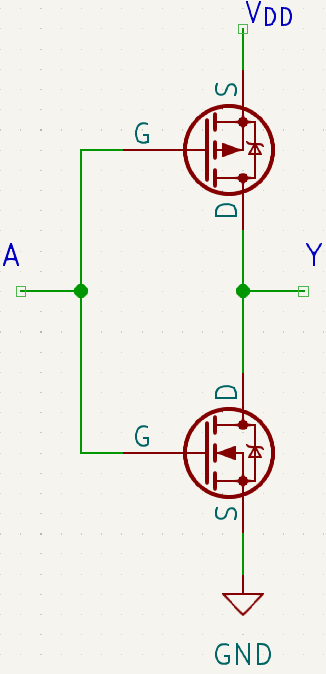
\includegraphics[width=0.5\textwidth]{MOSFET_logic/mosfet_not.png}
        \caption{MOSFETを用いたNOT回路}
        \label{fig:mosfet_not}
    \end{minipage}
    \begin{minipage}{0.55\hsize}
        \centering
        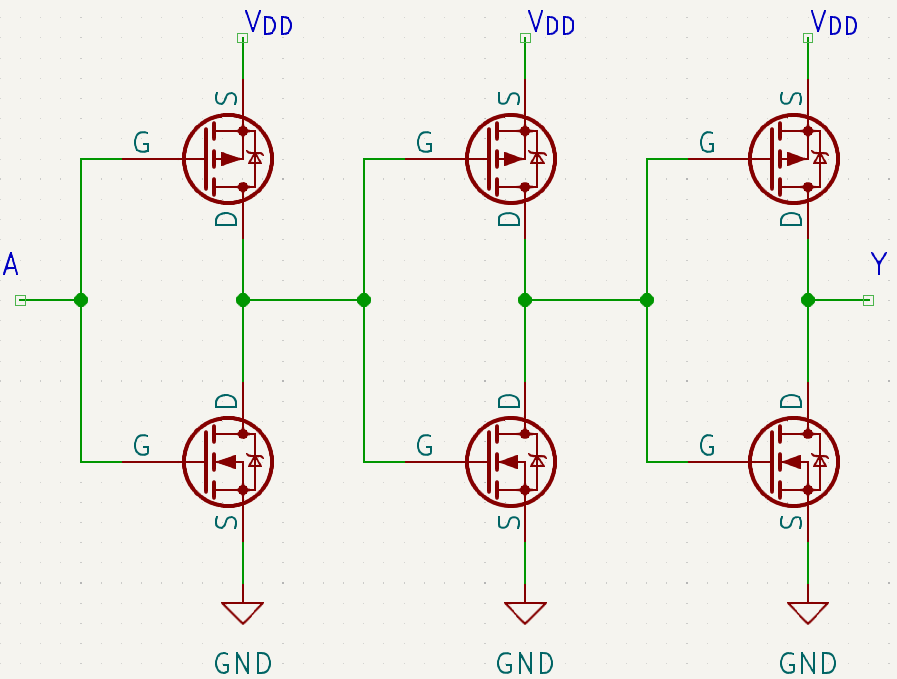
\includegraphics[width=0.9\textwidth]{MOSFET_logic/mosfet_not_real.png}
        \caption{実際のCMOSによるNOT回路}
        \label{fig:mosfet_not_real}
    \end{minipage}

\end{figure}

この回路は、PMOSトランジスタとNMOSトランジスタを組み合わせた回路であり、Complementary MOS (CMOS) 回路と呼ばれる。
復習であるが,Nch MOSFETはゲートにソースより高い電圧が印加されるとオンになる特性を持ち、Pch MOSFETはゲートにソースより低い電圧が印加されるとオンになる特性を持つ。
この回路において、入力が高電位（論理1）の場合、下側のNMOSトランジスタがオンになり、上側にPMOSトランジスタがオフになるため、出力はグランドに接続され、低電位（論理0）となる。
一方、入力が低電位（論理0）の場合、上側のPMOSトランジスタがオンになり、下側のNMOSトランジスタがオフになるため、出力は電源に接続され、高電位（論理1）となる。
このように、図\ref{fig:mosfet_not}の回路はNOT回路として動作する。

このCMOS回路の利点として、MOSFETを使用しているため、入力にほとんど電流が流れないため、入力インピーダンスが非常に高いことが挙げられる。
また、出力インピーダンスも低いため、他の回路への駆動能力が高い。
一方で、デメリットとして、MOSFETのゲートに電荷をチャージする時間だけ遅延が発生するため、スイッチング速度がBJTに比べて遅いこと、
静電気に弱いため、取り扱いに注意が必要であること、ONからOFFへの遷移時に一瞬両方のMOSFETがオンになるため、短時間ながらも電源からグランドに大きな電流が流れることが挙げられる。

なお実際のCMOSによるNOT回路では、図\ref{fig:mosfet_not_real}のように、図\ref{fig:mosfet_not}の回路を3個つなげて使っていることが多い。
% \begin{figure}[htbp]
%     \centering
%     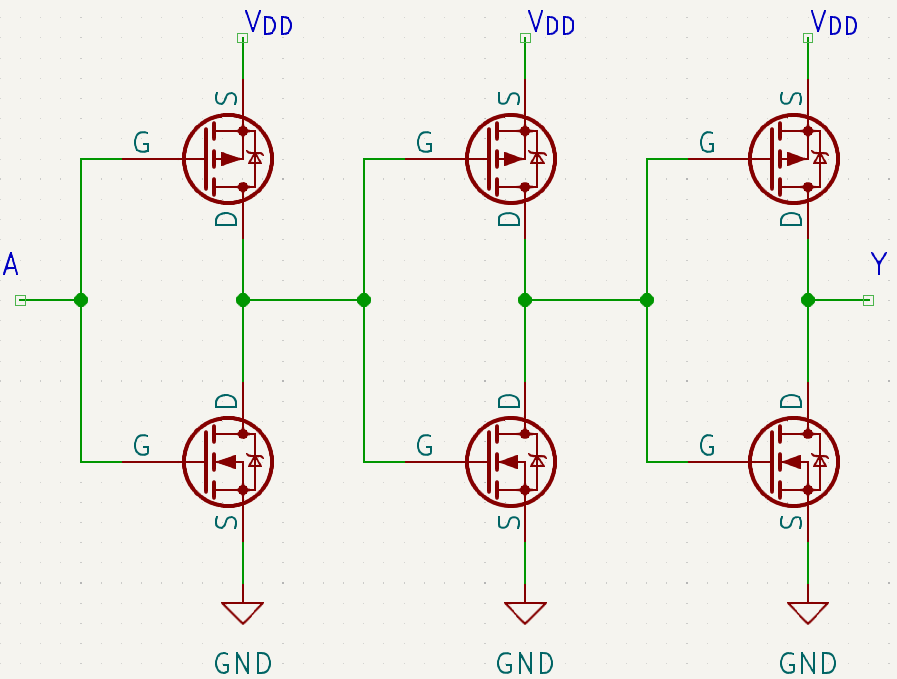
\includegraphics[width=0.5\textwidth]{MOSFET_logic/mosfet_not_real.png}
%     \caption{実際のCMOSによるNOT回路}
%     \label{fig:mosfet_not_real}
% \end{figure}

まず、図\ref{fig:mosfet_not}の回路はNOT回路を3つ直列につなげているため、出力もNOT回路となることがわかる。
これは、NOT回路の遅延時間等の特性をほかの論理回路と合わせるためであり、このような処理をした出力をバッファード出力と呼ぶ。

\newpage

次に、図\ref{fig:mosfet_nand}の回路を考えよう。
\begin{figure}[htbp]
    \centering
    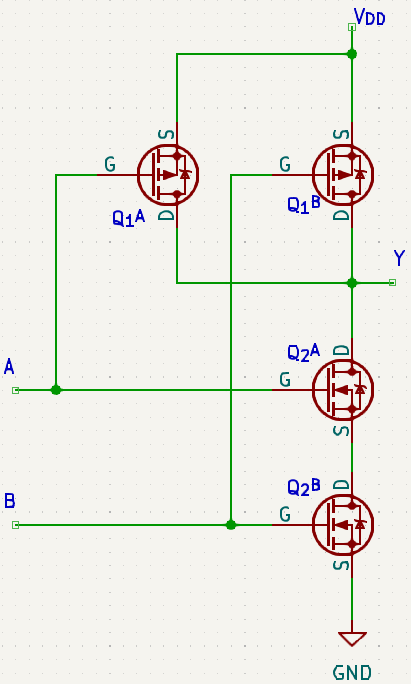
\includegraphics[width=0.4\textwidth]{MOSFET_logic/mosfet_nand.png}
    \caption{MOSFETを用いたNAND回路}
    \label{fig:mosfet_nand}
\end{figure}
この回路は、2つのPMOSトランジスタと2つのNMOSトランジスタを組み合わせた回路であり、NAND回路として動作する。
動作を確認しよう。
まず、入力Aが低電位(L)で、入力Bが低電位(L)の場合、$Q_1^A$と$Q_1^B$がオンになり、$Q_2^A$と$Q_2^B$がオフになるため、出力は電源に接続され、高電位(H)となる。
次に、入力Aが低電位(L)で、入力Bが高電位(H)の場合、$Q_1^A$と$Q_2^B$がオンになり、$Q_1^B$と$Q_2^A$がオフになるため、出力は電源に接続され、高電位(H)となる。
同様に、入力Aが高電位(H)で、入力Bが低電位(L)の場合も、出力は高電位(H)となる。
最後に、入力Aが高電位(H)で、入力Bが高電位(H)の場合、$Q_2^A$と$Q_2^B$がオンになり、$Q_1^A$と$Q_1^B$がオフになるため、出力はグランドに接続され、低電位(L)となる。
このように、図\ref{fig:mosfet_nand}の回路はNAND回路として動作する。

AND回路はNAND回路の出力をNOT回路(図\ref{fig:mosfet_not})に入力することで実現できるほか、NOR回路やOR回路も同様にして実現できる。
図\ref{fig:mosfet_all}の回路はそれぞれNOT回路、NAND回路、AND回路、NOR回路、OR回路をMOSFETで実現したものである。
特に動作原理を解説することはしないが、NAND回路の時と同じ考えで動作原理を確認することができるので、各自で確認してほしい.

\begin{figure}[htbp]
    \centering
    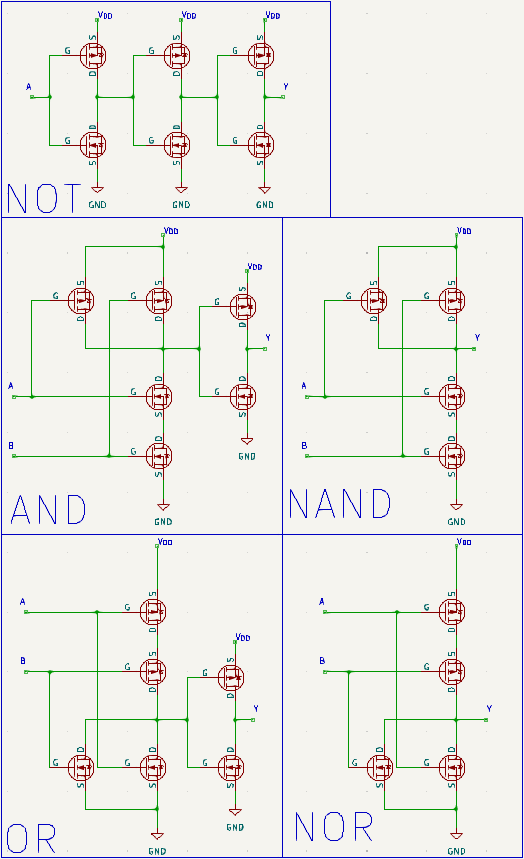
\includegraphics[width=0.95\textwidth]{MOSFET_logic/mosfet_all.png}
    \caption{MOSFETを用いた各種論理回路}
    \label{fig:mosfet_all}
\end{figure}
\newpage

以上のように、MOSFETを用いた論理回路はBJTを用いた論理回路と同様に動作するが、MOSFETの特性を活かした高入力インピーダンスや低出力インピーダンス,
出力電圧が完全に0Vまたは$V_{DD}$になることなどの利点があるため、現在ではMOSFETを用いた論理回路が主流となっている。

一方で、大きな弱点として、静電気に弱いことが挙げられる。
MOSFETのゲートは非常に薄い酸化膜で覆われており、静電気によってこの酸化膜が破壊されると、MOSFETが正常に動作しなくなる可能性がある。
そのため、多くの論理ゲートには静電気防止用の回路が組み込まれている。(図\ref{fig:esd_protection})

\begin{figure}[htbp]
    \centering
    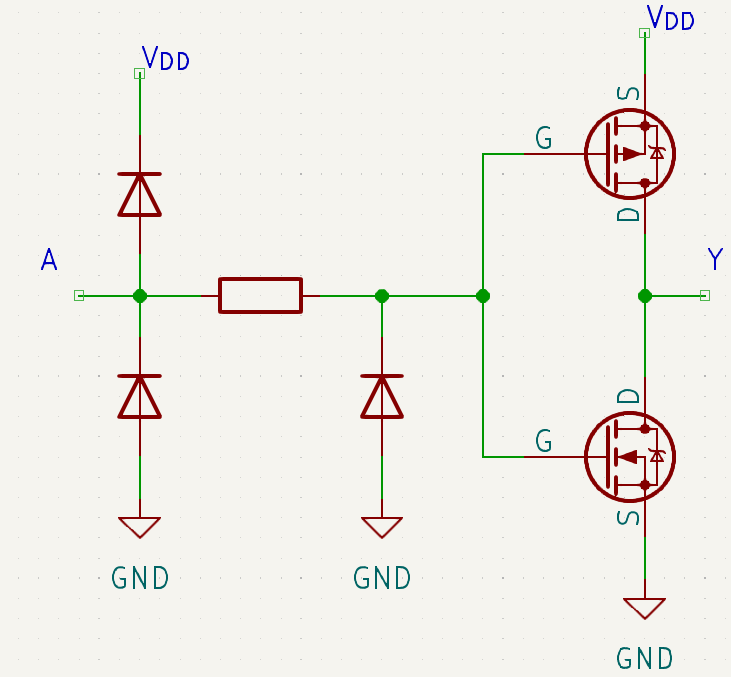
\includegraphics[width=0.5\textwidth]{MOSFET_logic/esd_protection.png}
    \caption{静電気防止回路の例}
    \label{fig:esd_protection}
\end{figure}

図\ref{fig:esd_protection}の回路では、入力端子に対して、$V_{DD}$とGNDにそれぞれダイオードが接続されている。
これにより、数万V程度にも及ぶ静電気が入力端子に加わった場合、電圧が正であっても負であってもダイオードが順方向に導通し、静電気を$V_{DD}$またはGNDに逃がすことで、MOSFETのゲートを保護している。
これで静電気によるMOSFETの破壊を防ぐことができるが、このダイオードは定常的に電流を流す設計になっていないので、
入力端子に$V_{DD}$より高い電圧を加えること、GNDより低い電圧を加えることは、論理回路の破壊の原因となるため、注意が必要である。

また、同様に、理論の章で説明したように、MOSFETには寄生ダイオードが存在するため、出力端子に$V_{DD}$より高い電圧を加えること、GNDより低い電圧を加えることも、論理回路の破壊の原因となるため、注意が必要である。


